\documentclass[tikz,border=3mm,multi=tikzpicture]{standalone}
\usepackage[utf8]{inputenc}
\usepackage[T1]{fontenc}
\usepackage{helvet}
\renewcommand{\familydefault}{\sfdefault}
\usepackage{tikz}
\usetikzlibrary{arrows.meta,calc,positioning}
\begin{document}

\tikzset{every node/.append style={font=\sffamily\small}}

% TikZ 1
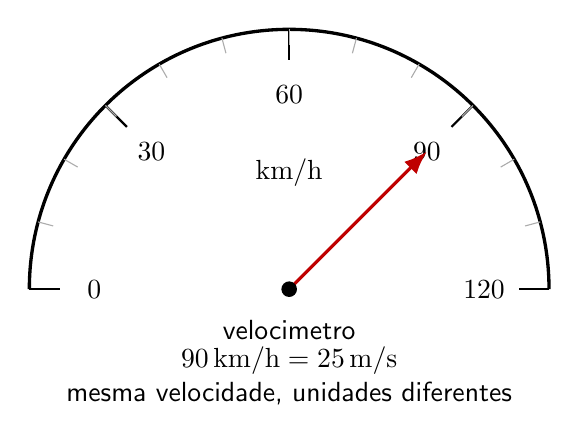
\begin{tikzpicture}[scale=1.1,>=Latex]
  \draw[very thick] (-3,0) arc[start angle=180,end angle=0,radius=3];
  \foreach \ang/\lab in {180/0,135/30,90/60,45/90,0/120}{
    \draw[thick] ({3*cos(\ang)},{3*sin(\ang)}) -- ({2.65*cos(\ang)},{2.65*sin(\ang)});
    \node at ({2.25*cos(\ang)},{2.25*sin(\ang)}) {$\lab$};
  }
  \foreach \ang in {165,150,...,15}{
    \draw[gray!65] ({3*cos(\ang)},{3*sin(\ang)}) -- ({2.82*cos(\ang)},{2.82*sin(\ang)});
  }
  \draw[very thick,red!75!black,->] (0,0) -- ({2.25*cos(45)},{2.25*sin(45)});
  \fill (0,0) circle (0.09);
  \node[below] at (0,-0.25) {velocimetro};
  \node[align=center] at (0,-1.0) {$90\,\mathrm{km/h}=25\,\mathrm{m/s}$\\mesma velocidade, unidades diferentes};
  \node at (0,1.35) {$\mathrm{km/h}$};
\end{tikzpicture}

% TikZ 2
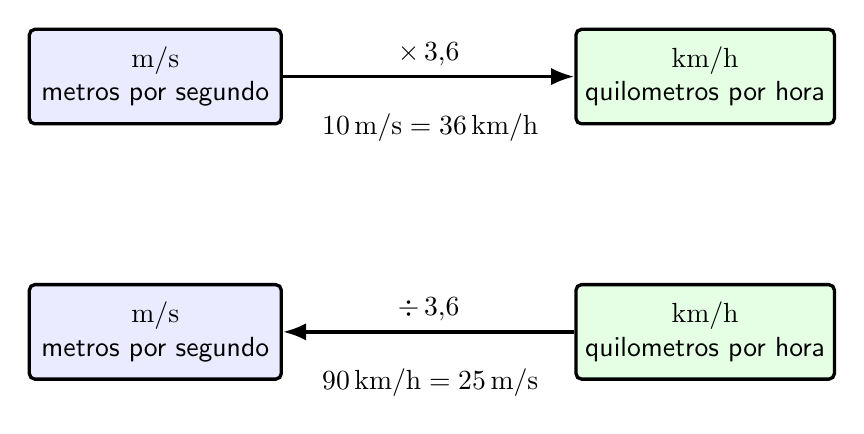
\begin{tikzpicture}[>=Latex,node distance=1.4cm]
  \tikzstyle{unitbox}=[draw,rounded corners=2pt,minimum width=3.2cm,minimum height=1.2cm,align=center,very thick]
  \node[unitbox,fill=blue!8] (ms1) {$\mathrm{m/s}$\\metros por segundo};
  \node[unitbox,fill=green!10,right=3.7cm of ms1] (kmh1) {$\mathrm{km/h}$\\quilometros por hora};
  \draw[very thick,->] (ms1) -- node[above] {$\times\,3{,}6$} (kmh1);
  \node[below=0.35cm of $(ms1)!0.5!(kmh1)$] {$10\,\mathrm{m/s}=36\,\mathrm{km/h}$};

  \node[unitbox,fill=green!10,below=2.0cm of kmh1] (kmh2) {$\mathrm{km/h}$\\quilometros por hora};
  \node[unitbox,fill=blue!8,left=3.7cm of kmh2] (ms2) {$\mathrm{m/s}$\\metros por segundo};
  \draw[very thick,->] (kmh2) -- node[above] {$\div\,3{,}6$} (ms2);
  \node[below=0.35cm of $(ms2)!0.5!(kmh2)$] {$90\,\mathrm{km/h}=25\,\mathrm{m/s}$};
\end{tikzpicture}

\end{document}
